% Writen by Jie Yin of NENU in Jan,27 2023.
% Utf-8. Xelatex(makeindex) - biber - Xelatex - Xelatex.

\documentclass{ctexart}
% \documentclass[zihao = -4]{ctexart} % scheme=chinese时,字号默认为五号。-4指小四。
% linespread = 1.3。对标准文档类初始值为1.3,即1.3倍行距。
% 此时,相邻两行的基线(\baselineskip)距离为1.3 × 1.2 = 1.56 倍字体高度。
% biblatex宏包使用biber编译

\usepackage{geometry} % 调整页面格式
\usepackage{graphicx} % 插入图片
\usepackage{color}    % 提供颜色
\usepackage{xcolor}   % 提供颜色
\usepackage{amsmath}  % 提供一些符号
\usepackage{amssymb}  % 多提供一些符号
\usepackage{amsthm}   % 丰富定理环境
\usepackage{bm}		  % 提供一些加粗环境,在rmd中可能与Unicode类宏包冲突
\usepackage{booktabs} % 三线表
\usepackage{longtable} % 长表格
\usepackage{caption}  % caption和图表间留出间距
\usepackage{listings} % 代码
\usepackage{imakeidx} % 插入索引。若用makeix宏包需要手动编译。

% 同时调用gb7714-2015.bbx 和gb7714-2015.cbx 使用符合GB/T 7714-2015 规范的参考文献样式
\usepackage[style=gb7714-2015]{biblatex}
% 著录样式调用gb7714-2015.bbx,引用样式调用biblatex 宏包自带的authoryear
% \usepackage[bibstyle=gb7714-2015,citestyle=authoryear]{biblatex}
% style=caspervector 以中文文献著录标准GB/T 7714—2015 为基础的一个样式。

\usepackage{hyperref} % 加超链接,最好最后调用,防止报错

\addbibresource{bibtest.bib} % 指定bib文件。注意加.bib 扩展名。
\pagestyle{plain} % 页眉为空,页脚为页码。ctex默认为"heading",即页眉为章节标题和页码,页脚为空。
\geometry{a4paper,left=1.25in,right=1.25in,top=1in,bottom=1in} % 符合Microsoft Word 习惯的页面设定是A4 纸张,上下边距1 英寸,左右边距1.25英寸 
\hypersetup{hidelinks} % 令超链接不带颜色也不带边框
\graphicspath{{figures/}} % 设置图片的子目录
\indexsetup{noclearpage}  % 索引不产生新页

% amsthm 提供了\theoremstyle 命令支持定理格式的切换。并提供了不带编号的*环境。
\theoremstyle{plain} 		     % 粗体标签、斜体内容
\newtheorem{theorem}{定理}[section]
\newtheorem{lemma}{引理}[section]
\newtheorem{corollary}{推论}[section]
\newtheorem{proposition}{命题}[section]
\newtheorem{conjecture}{推测}[section]

\theoremstyle{definition} 		 % 粗体标签、正体内容
\newtheorem{definition}{定义}[section]
\newtheorem{example}{例子}[section]
\newtheorem{exercise}{练习}[section]
\newtheorem{hypothesis}{假设}[section]

\theoremstyle{remark} 			 % 斜体标签、正体内容
\newtheorem*{remark}{注}
\newtheorem*{solution}{解}

% 调整section对应标题为 类似'第一章'的格式
\ctexset{
	section/name = {第,章},                  
	section/number = {\chinese{section}},
	appendix/name= {附录}
}
% 代码环境使用某种字体,设置关键字颜色,注释颜色,背景框颜色
\lstset{
	basicstyle=\tt,                            
	keywordstyle=\color{purple}\bfseries,
	commentstyle=\color{gray},
	backgroundcolor=\color[RGB]{245,245,244},
}

% 创建新环境Highlighting,用于展示R codes。
\usepackage{fancyvrb}	   
\newcommand{\VerbBar}{|}
\newcommand{\VERB}{\Verb[commandchars=\\\{\}]}
\DefineVerbatimEnvironment{Highlighting}{Verbatim}{commandchars=\\\{\}}
% Add ',fontsize=\small' for more characters per line

% 创建新环境Shaded,用于展示R codes.
\usepackage{framed}			
\definecolor{shadecolor}{RGB}{248,248,248}  % 代码块背景颜色
\newenvironment{Shaded}{\begin{snugshade}}{\end{snugshade}}

% 新环境Highlighting的关键词对应的颜色
\newcommand{\AlertTok}[1]{\textcolor[rgb]{0.94,0.16,0.16}{#1}}
\newcommand{\AnnotationTok}[1]{\textcolor[rgb]{0.56,0.35,0.01}{\textbf{\textit{#1}}}}
\newcommand{\AttributeTok}[1]{\textcolor[rgb]{0.77,0.63,0.00}{#1}}
\newcommand{\BaseNTok}[1]{\textcolor[rgb]{0.00,0.00,0.81}{#1}}
\newcommand{\BuiltInTok}[1]{#1}
\newcommand{\CharTok}[1]{\textcolor[rgb]{0.31,0.60,0.02}{#1}}
\newcommand{\CommentTok}[1]{\textcolor[rgb]{0.56,0.35,0.01}{\textit{#1}}}
\newcommand{\CommentVarTok}[1]{\textcolor[rgb]{0.56,0.35,0.01}{\textbf{\textit{#1}}}}
\newcommand{\ConstantTok}[1]{\textcolor[rgb]{0.00,0.00,0.00}{#1}}
\newcommand{\ControlFlowTok}[1]{\textcolor[rgb]{0.13,0.29,0.53}{\textbf{#1}}}
\newcommand{\DataTypeTok}[1]{\textcolor[rgb]{0.13,0.29,0.53}{#1}}
\newcommand{\DecValTok}[1]{\textcolor[rgb]{0.00,0.00,0.81}{#1}}
\newcommand{\DocumentationTok}[1]{\textcolor[rgb]{0.56,0.35,0.01}{\textbf{\textit{#1}}}}
\newcommand{\ErrorTok}[1]{\textcolor[rgb]{0.64,0.00,0.00}{\textbf{#1}}}
\newcommand{\ExtensionTok}[1]{#1}
\newcommand{\FloatTok}[1]{\textcolor[rgb]{0.00,0.00,0.81}{#1}}
\newcommand{\FunctionTok}[1]{\textcolor[rgb]{0.00,0.00,0.00}{#1}}
\newcommand{\ImportTok}[1]{#1}
\newcommand{\InformationTok}[1]{\textcolor[rgb]{0.56,0.35,0.01}{\textbf{\textit{#1}}}}
\newcommand{\KeywordTok}[1]{\textcolor[rgb]{0.13,0.29,0.53}{\textbf{#1}}}
\newcommand{\NormalTok}[1]{#1}
\newcommand{\OperatorTok}[1]{\textcolor[rgb]{0.81,0.36,0.00}{\textbf{#1}}}
\newcommand{\OtherTok}[1]{\textcolor[rgb]{0.56,0.35,0.01}{#1}}
\newcommand{\PreprocessorTok}[1]{\textcolor[rgb]{0.56,0.35,0.01}{\textit{#1}}}
\newcommand{\RegionMarkerTok}[1]{#1}
\newcommand{\SpecialCharTok}[1]{\textcolor[rgb]{0.00,0.00,0.00}{#1}}
\newcommand{\SpecialStringTok}[1]{\textcolor[rgb]{0.31,0.60,0.02}{#1}}
\newcommand{\StringTok}[1]{\textcolor[rgb]{0.31,0.60,0.02}{#1}}
\newcommand{\VariableTok}[1]{\textcolor[rgb]{0.00,0.00,0.00}{#1}}
\newcommand{\VerbatimStringTok}[1]{\textcolor[rgb]{0.31,0.60,0.02}{#1}}
\newcommand{\WarningTok}[1]{\textcolor[rgb]{0.56,0.35,0.01}{\textbf{\textit{#1}}}}

\makeindex[columns=2, intoc, columnseprule] % 开始记录索引。分两栏,两栏中有横线,并在目录中显示

\title{我的CTeX模板}
\author{尹杰}
\date{\today}

\begin{document}

\maketitle % 生成标题

\section*{摘要}
如果你有意在这份文档中增加、删除或者改变一些内容,请通知作者。作者对\LaTeX 初学者
的反馈特别感兴趣,尤其是关于这份介绍哪些内容很容易理解,哪些内容可能需要更好地解释,
而哪些内容由于太过难以理解、非常不常用而不适宜放在本手册。
\vspace{0.5ex} % 与下一行空一点距离

{\heiti \bfseries {\large 关键词:}\ 支持向量机,\ 二分类模型,
		\  预订取消检测,\ \itshape Mlr3verse}

\newpage		 % 新的一页
\tableofcontents % 生成目录

\newpage		 % 新的一页

\part{部分}
图片见第\ref{sec:fig}章。公式见\ref{subsec:equ}节。

部分下的正文。部分下的正文。部分下的正文。部分下的正文。部分下的正文。部分下的正文。部分下的正文。部分下的正文。部分下的正文。部分下的正文。部分下的正文。部分下的正文。部分下的正文。部分下的正文。部分下的正文。部分下的正文。部分下的正文。部分下的正文。部分下的正文。部分下的正文。部分下的正文。部分下的正文。

\section{章}
标题下的正文。标题下的正文。标题下的正文。标题下的正文。标题下的正文。标题下的正文。标题下的正文。标题下的正文。标题下的正文。标题下的正文。标题下的正文。标题下的正文。标题下的正文。标题下的正文。标题下的正文。标题下的正文。标题下的正文。标题下的正文。标题下的正文。标题下的正文。标题下的正文。标题下的正文。

\subsection{节}
{\small The small and
	\textbf{bold} Romans ruled} % \bfseries \textbf

{\large all of great big
	{\itshape Italy}.} % \itshape \textit

An \underline{underlined} text.

试着加一个索引\verb|\index{aaa}|\index{aaa}。

节下的正文。节下的正文。节下的正文。节下的正文。节下的正文。节下的正文。节下的正文。节下的正文。节下的正文。节下的正文。节下的正文。节下的正文。节下的正文。节下的正文。节下的正文。节下的正文。节下的正文。节下的正文。节下的正文。节下的正文。节下的正文。节下的正文。节下的正文。节下的正文。节下的正文。节下的正文。\footnote{来个脚注}

\subsection{小节}
小节下的正文。小节下的正文。小节下的正文。小节下的正文。小节下的正文。小节下的正文。小节下的正文。小节下的正文。小节下的正文。小节下的正文。小节下的正文。小节下的正文。小节下的正文。小节下的正文。小节下的正文。小节下的正文。小节下的正文。小节下的正文。小节下的正文。小节下的正文。小节下的正文。小节下的正文。

顺便介绍一下引用环境。木兰诗:
\begin{quotation}
	万里赴戎机,关山度若飞。
	朔气传金柝,寒光照铁衣。
	将军百战死,壮士十年归。
	归来见天子,天子坐明堂。
	策勋十二转,赏赐百千强。
\end{quotation}

\paragraph{段落}
段落下的正文。段落下的正文。段落下的正文。段落下的正文。段落下的正文。段落下的正文。段落下的正文。段落下的正文。段落下的正文。段落下的正文。段落下的正文。段落下的正文。段落下的正文。段落下的正文。段落下的正文。段落下的正文。段落下的正文。段落下的正文。段落下的正文。段落下的正文。段落下的正文。段落下的正文。

\subparagraph{子段落}
子段落下的正文。子段落下的正文。子段落下的正文。子段落下的正文。子段落下的正文。子段落下的正文。子段落下的正文。子段落下的正文。子段落下的正文。子段落下的正文。子段落下的正文。子段落下的正文。子段落下的正文。子段落下的正文。子段落下的正文。子段落下的正文。子段落下的正文。子段落下的正文。子段落下的正文。

\subsubsection{序列最小最优化算法(SMO)}
下面再多写一点试一下。

SMO的基本思路是先固定$\alpha_{i}$之外的所有参数,然后求定$\alpha_{i}$上的极值。由于存在约束$\sum_{i=1}^N{\alpha _iy_i}=0$,若固定$\alpha_{i}$之外的其他变量,则$\alpha_{i}$可由其他变量导出。于是,SMO每次选择两个变量$\alpha_{i}$和$\alpha_{j}$, 并固定其他参数。这样,在参数初始化后,SMO不断执行如下两个步骤直至收敛:
\begin{itemize}
	\item 选取一对需更新的变量$\alpha_{i}$和$\alpha_{j}$
	\item 固定$\alpha_{i}$和$\alpha_{j}$以外的参数,获得更新后的$\alpha_{i}$和$\alpha_{j}$
\end{itemize}

一种直观的解释是,这样的两个变量有很大的差别,与对两个相似的变量进行更新相比,对它们进行更新会带给目标函数值更大的变化。SMO算法之所以高效,恰由于在固定其他参数后,仅优化两个参数的过程能做到非常高效。
约束可以重写为式\verb|\eqref{eq:1}| \eqref{eq:1}:
\begin{equation}
	\alpha _i y_i+\alpha _j y_j = c,\quad \alpha _i\geqslant 0,\quad \alpha _j\geqslant 0
	\label{eq:1}
\end{equation}

\section{图片} \label{sec:fig}
\LaTeX 预定义了两类浮动体环境figure 和table。习惯上figure 里放图片,table 里放
表格,但并没有严格限制,可以在任何一个浮动体里放置文字、公式、表格、图片等等任意内容。
\index{aab}

我们时常有在一个浮动体里面放置多张图的用法。最简单的用法就是直接并排放置,也可以
通过分段或者换行命令\verb|\\| 排版多行多列的图片,以下为示意代码。
\begin{verbatim}
	\begin{figure}[htbp]
		\centering
		\includegraphics[width=...]{...}
		\qquad
		\includegraphics[width=...]{...} \\[...pt]
		\includegraphics[width=...]{...}
		\caption{...}
	\end{figure}
\end{verbatim}

由于标题是横跨一行的,用\verb|\caption| 命令为每个图片单独生成标题就需要借助前文提到的
\verb|\parbox| 或者minipage 环境,将标题限制在盒子内。

下面画了图\ref{fig1},\ref{fig2}和\ref{fig3}。
\begin{figure}[htbp]
	\centering
	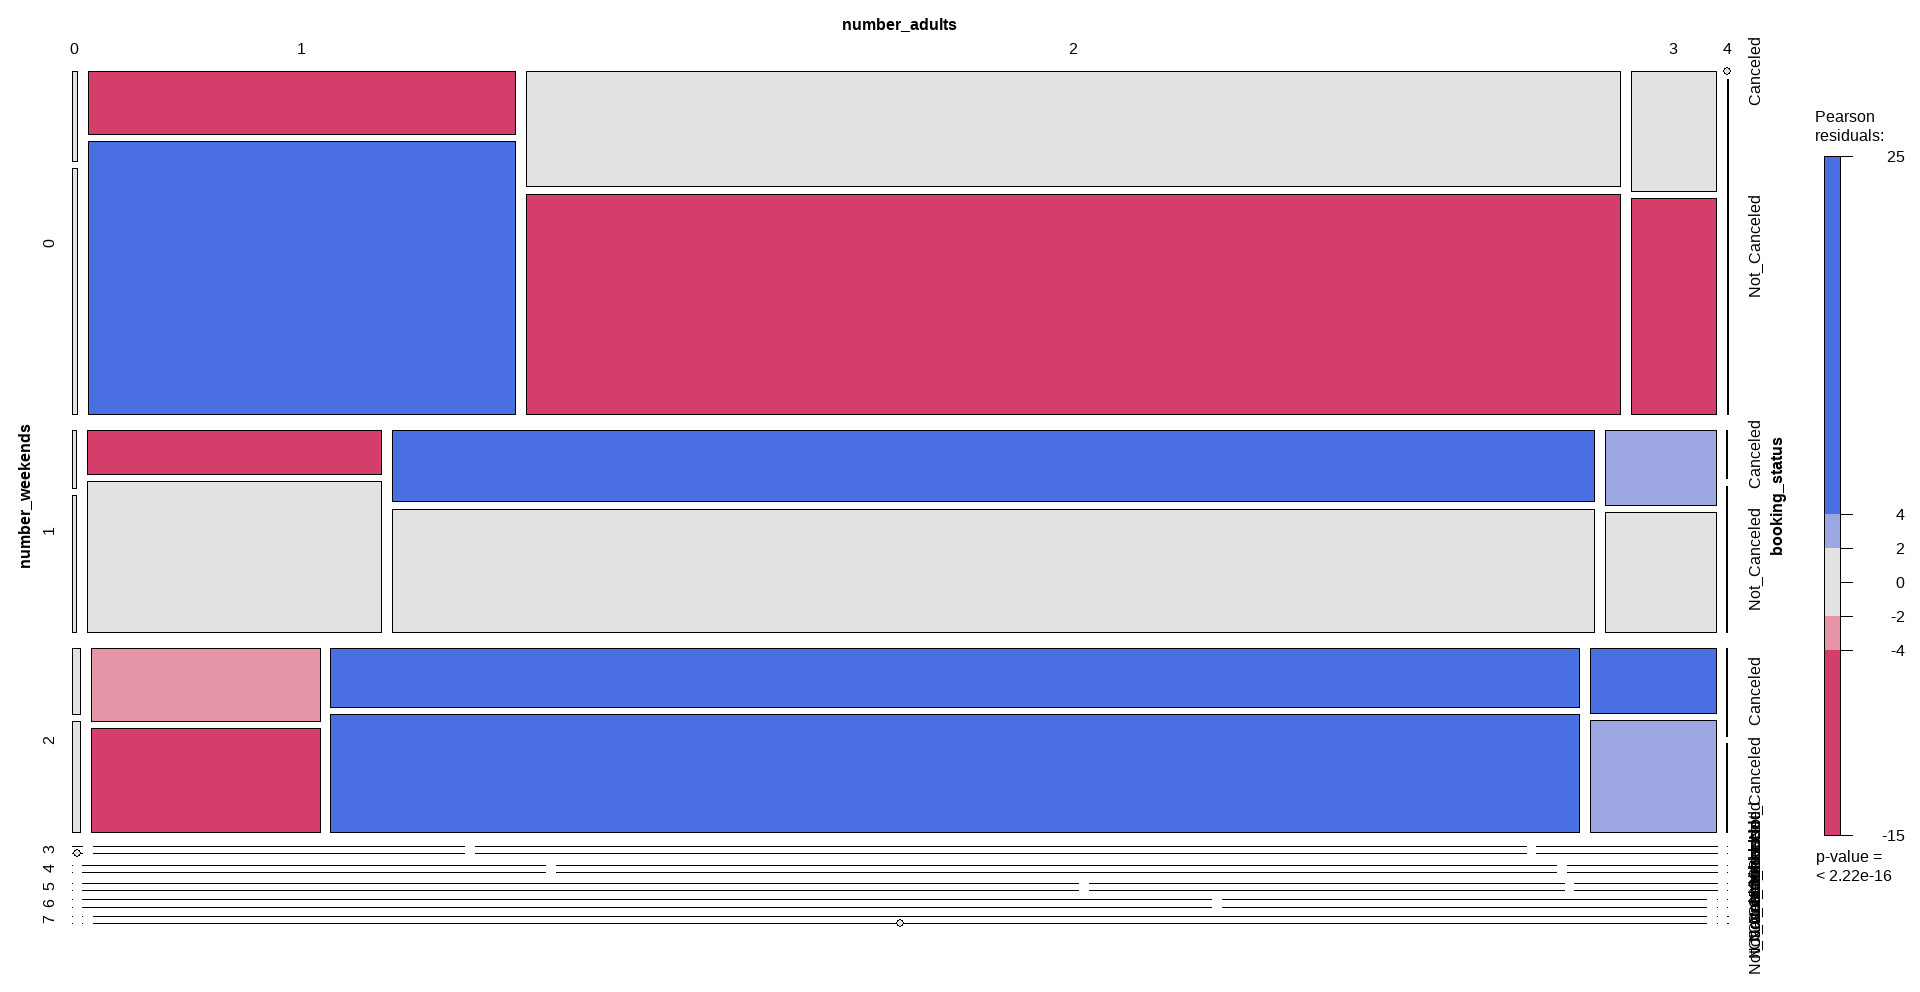
\includegraphics[width=1\textwidth]{fig1}
	\caption{一张图}
	\label{fig1}
\end{figure}

\begin{figure}[htbp]
	\centering
	\begin{minipage}{12em}
		\centering
		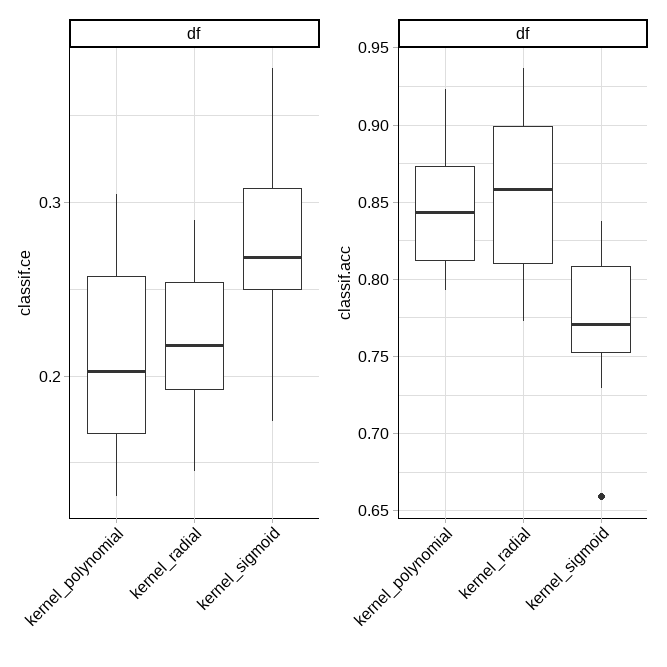
\includegraphics[width=1\textwidth]{fig2}
		\caption{并排图左}\label{fig2}
	\end{minipage}
	\qquad
	\begin{minipage}{12em}
		\centering
		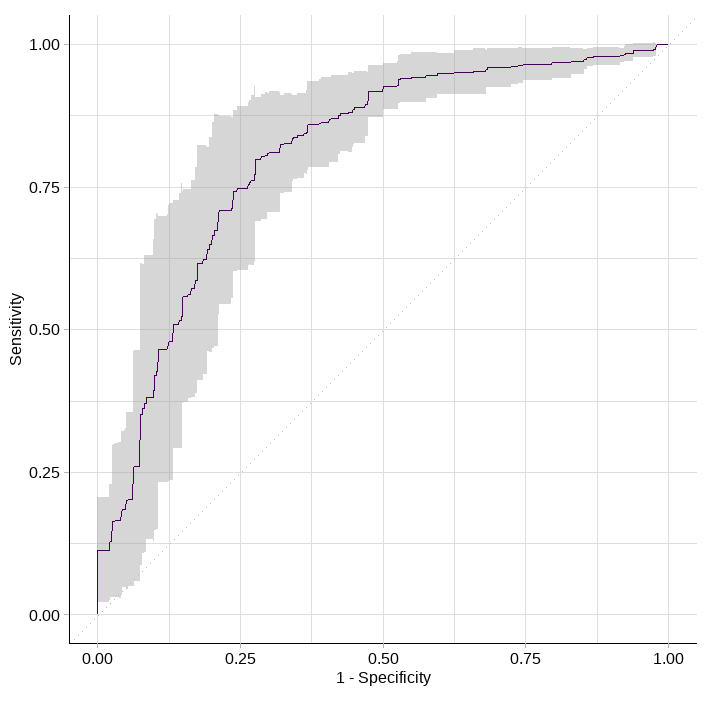
\includegraphics[width=1\textwidth]{fig3}
		\caption{并排图2右}\label{fig3}
	\end{minipage}
\end{figure}

\section{表格}
来个表\ref{tab:1}。\index{ac}

\begin{table}[htbp]
	\centering
	\caption{一张表}
	\label{tab:1}
	\begin{tabular}{cccc}
		\toprule
		& \multicolumn{3}{c}{Numbers} \\
		\cmidrule{2-4}
		& 1 & 2 & 3 \\
		\midrule
		Alphabet & A & B & C \\
		Roman & I & II& III \\
		\bottomrule
	\end{tabular}
\end{table}

看看\hyperref[item]{项目列表}
\begin{enumerate}
	\label{item}
	\item An item.
	\begin{enumerate}
		\item A nested item.\label{itref}
		\item[*] A starred item.
		\item  One more item.
	\end{enumerate}
	\item Reference(\ref{itref}).
\end{enumerate}

\index{bbb}

\begin{description}
	\item[强调一下] Numbered list.
	\item[再强调一下] Non-numbered list.
\end{description}

\section{定理什么的}
\index{ccc}
\begin{theorem}[可以在中括号里写]
	\label{the:1}
	一个定理。
\end{theorem}

\begin{lemma}[引理1]
	\label{lem:1}
	一个引理。
\end{lemma}

\begin{definition}
	\label{def:1}
	一个定义。
\end{definition}

\begin{remark}
	一条评论。
\end{remark}

可以引用定理\ref{the:1}和引理\ref{lem:1}和定义\ref{def:1}。还有一些其他的:
\begin{description}
	\item[粗体标签、斜体内容] 定理theorem,引理lemma,推论corollary,命题proposition,推测conjecture
	\item[粗体标签、正体内容] 定义definition,例子example,练习exercise,假设hypothesis
	\item[斜体标签、正体内容] 注remark,解solution
\end{description}

amsthm 还提供了一个proof 环境用于排版定理的证明过程。proof 环境末尾自动加上一个
证毕符号。如果行末是一个不带编号的公式, 符号会另起一行,这时可使用\verb|\qedhere| 命令将符
号放在公式末尾。
\begin{proof}
	我们有质能公式:
	\[
	E=mc^2 \qedhere
	\]
\end{proof}

\section{一些其他的}
\subsection{公式} \label{subsec:equ}
\index{ddd}
\LaTeX 允许一部分数学符号切换字体,主要是拉丁字母、数字、大写希腊字母以及重音符号
等。某一些命令需要字体宏包的支持。

$\mathcal{R} \quad \mathfrak{R} \quad \mathbb{R}$

加粗\verb|\mathbf{A}| $\mathbf{A}$,倾斜\verb|\mathit{A}| $\mathit{A}$。如果想得到粗斜体,可以使用amsmath宏包提供的\verb|\boldsymbol| 命令$\boldsymbol{A}$。,一些符号本身并没有粗体版本,使用\verb|\boldsymbol| 也得不到粗体。
此时bm 宏包的\verb|\bm| 命令会生成“伪粗体”$\bm{\mu}$,尽管效果比较粗糙,但在某些时候也不失为一种解决方案。

多行公式目前最常用的是align 环境,它将公式用\& 隔为两部分并对齐。分隔符通常放在等号左边。align 环境会给每行公式都编号。我们仍然可以用\verb|\notag| 去掉某行的编号。
\begin{align}
	a ={} & b + c \\
	={} & d + e + f + g + h + i
	+ j + k + l \notag \\
	& + m + n + o \\
	={} & p + q + r + s
\end{align}

如果我们不需要按等号对齐,只需罗列数个公式,gather 将是一个很好用的环境。可以用\verb|\notag|使某行不编号。
\begin{gather}
	a = b + c \\
	d = e + f + g \\
	h + i = j + k \notag \\
	l + m = n
\end{gather}

另一个常见的需求是将多个公式组在一起公用一个编号,编号位于公式的居中位置。为此,
amsmath 宏包提供了诸如aligned、gathered 等环境,与equation 环境套用。
\begin{equation}
	\begin{aligned}
		a &= b + c \\
		d &= e + f + g \\
		h + i &= j + k \\
		l + m &= n
	\end{aligned}
\end{equation}

amsmath 宏包的multline 环境提供了书写折行长公式的方便环境。它允许用\\ 折行,将
公式编号放在最后一行。多行公式的首行左对齐,末行右对齐,其余行居中。
\begin{multline}
	a + b + c + d + e + f
	+ g + h + i \\
	= j + k + l + m + n\\
	= o + p + q + r + s\\
	= t + u + v + x + z
\end{multline}

我们当然也可以用array 环境排版各种矩阵。amsmath 宏包还直接提供了多种排版矩阵的
环境,包括不带定界符的matrix,以及带各种定界符的矩阵pmatrix等。用\verb|\[ \]|或\verb|$ $|默认不编号,在equation环境中默认编号,如式\eqref{eq-10}。
\[ \mathbf{X} = \left(
\begin{array}{cccc}
	x_{11} & x_{12} & \ldots & x_{1n}\\
	x_{21} & x_{22} & \ldots & x_{2n}\\
	\vdots & \vdots & \ddots & \vdots\\
	x_{n1} & x_{n2} & \ldots & x_{nn}\\
\end{array} \right) \]

\begin{equation}
	\begin{matrix}
		1 & 2 \\ 3 & 4
	\end{matrix} \qquad
	\begin{bmatrix}
		x_{11} & x_{12} & \ldots & x_{1n}\\
		x_{21} & x_{22} & \ldots & x_{2n}\\
		\vdots & \vdots & \ddots & \vdots\\
		x_{n1} & x_{n2} & \ldots & x_{nn}\\
	\end{bmatrix}
	\label{eq-10}
\end{equation}

\subsection{一些包}
\index{eee}
颜色也要记得用package哦。{\color{red} 红色}。这里用xcolor宏包。

还得用hyperref宏包为引用加上超链接。\href{bing.com}{Bing}。

\subsection{代码}
\index{eff}
还有代码。用listings宏包。但是不太好看。
\begin{lstlisting}[language=R]
	library(tidyverse)
	library(lubridate)
	library(skimr)
	
	# 试试注释和中文怎么样
	data = data_origin  %>% 
	mutate(across(c(type_of_meal_plan,
	required_car_parking_space,
	booking_status),as.factor))
\end{lstlisting}

或者用自定义的Shaded环境和Highlighting环境(从Rmarkdown移植)。代码要从Rmd生成的tex文件里面原封不动的粘贴过来,否则缩进可能发生混乱。
\begin{Shaded}
\begin{Highlighting}[]
\NormalTok{bookdown}\SpecialCharTok{::}\FunctionTok{render\_book}\NormalTok{(}\StringTok{"index.Rmd"}\NormalTok{, }
	\AttributeTok{output\_format=}\StringTok{"bookdown::gitbook"}\NormalTok{, }\AttributeTok{encoding=}\StringTok{"UTF{-}8"}\NormalTok{)}
\end{Highlighting}
\end{Shaded}


\subsection{参考文献}
再看看下面参考文献怎么整。

见文献\cite{sun}。见文献\citeauthor{sun}。见文献\citeyear{sun}。
见文献\textcite{sun}。见文献\parencite{sun}。

见文献\cite{zhang__2019}。见文献\citeauthor{zhang__2019}。见文献\citeyear{zhang__2019}。见文献\textcite{zhang__2019}。见文献\parencite{zhang__2019}。

见文献\cite{Blakeley}。见文献\citeauthor{Blakeley}。见文献\citeyear{Blakeley}。见文献\textcite{Blakeley}。见文献\parencite{Blakeley}。见文献\cite{sun,zhang__2019,Blakeley}和\citeauthor{sun,zhang__2019,Blakeley}。

时下许多学术期刊比较喜欢使用人名——年份的引用方式,形如(Axford et al., 2013)。natbib
宏包提供了对这种“自然”引用方式的处理。

\verb|\usepackage[numbers,sort&compress]{natbib}| 。natbib宏包同样也支持数字引用,并且支持将引用的序号压缩。\verb|\citep{zhang__2019}| 和
\verb|\citet{zhang__2019}|。

\newpage
\nocite{*}				 % 没引用的文献也打印
\printbibliography   	 % 参考文献

\newpage
\appendix				 % 之后的章节视为附录。默认以ABCD为序号。
\section{试试放个附录}
附录的内容在\verb|\appendix|之后再用section。

\subsection{子附录}
也可以用subsection

\section{再来个附录}
附录的内容。附录的内容。附录的内容。附录的内容。附录的内容。附录的内容。附录的内容。附录的内容。附录的内容。附录的内容。附录的内容。附录的内容。附录的内容。附录的内容。附录的内容。附录的内容。附录的内容。附录的内容。附录的内容。附录的内容。附录的内容。附录的内容。附录的内容。

\newpage
\listoffigures			 % 图目录
\addcontentsline{toc}{section}{插图} % 将图目录作为一章加入总目录
\listoftables			 % 表目录
\addcontentsline{toc}{section}{表格} % 将表目录作为一章加入总目录

\indexprologue{这里是索引的一些说明文字.可选项为间隔长度,默认为bigskip。索引的排序是按照ABCD的字母序排列的。} % 生成索引说明文字
\printindex				 % 生成索引
\end{document}
